\parindent=0em
\subsection{DAQRI Smart Helmet}
\label{HoloLens2Dispositivo}
\noindent

%https://www.linkedin.com/pulse/daqri-smart-helmet-closer-look-nathan-gaydhani

El \textit{DAQRI Smart Helmet} es un dispositivo de realidad mixta estereoscópico sin cables integrado en un casco duro (cascos utilizados por ejemplo en la construcción). Es por esto por lo que está centrado en usos industriales, además, contiene un alto número de sensores para facilitar su uso sin manos.\\

Este casco tiene un peso total de 1 kilo y 500 gramos, tres veces el peso de las Hololens 2 (sección {\ref{HoloLens2Dispositivo}}).


\begin{figure}[h]
    \centering
    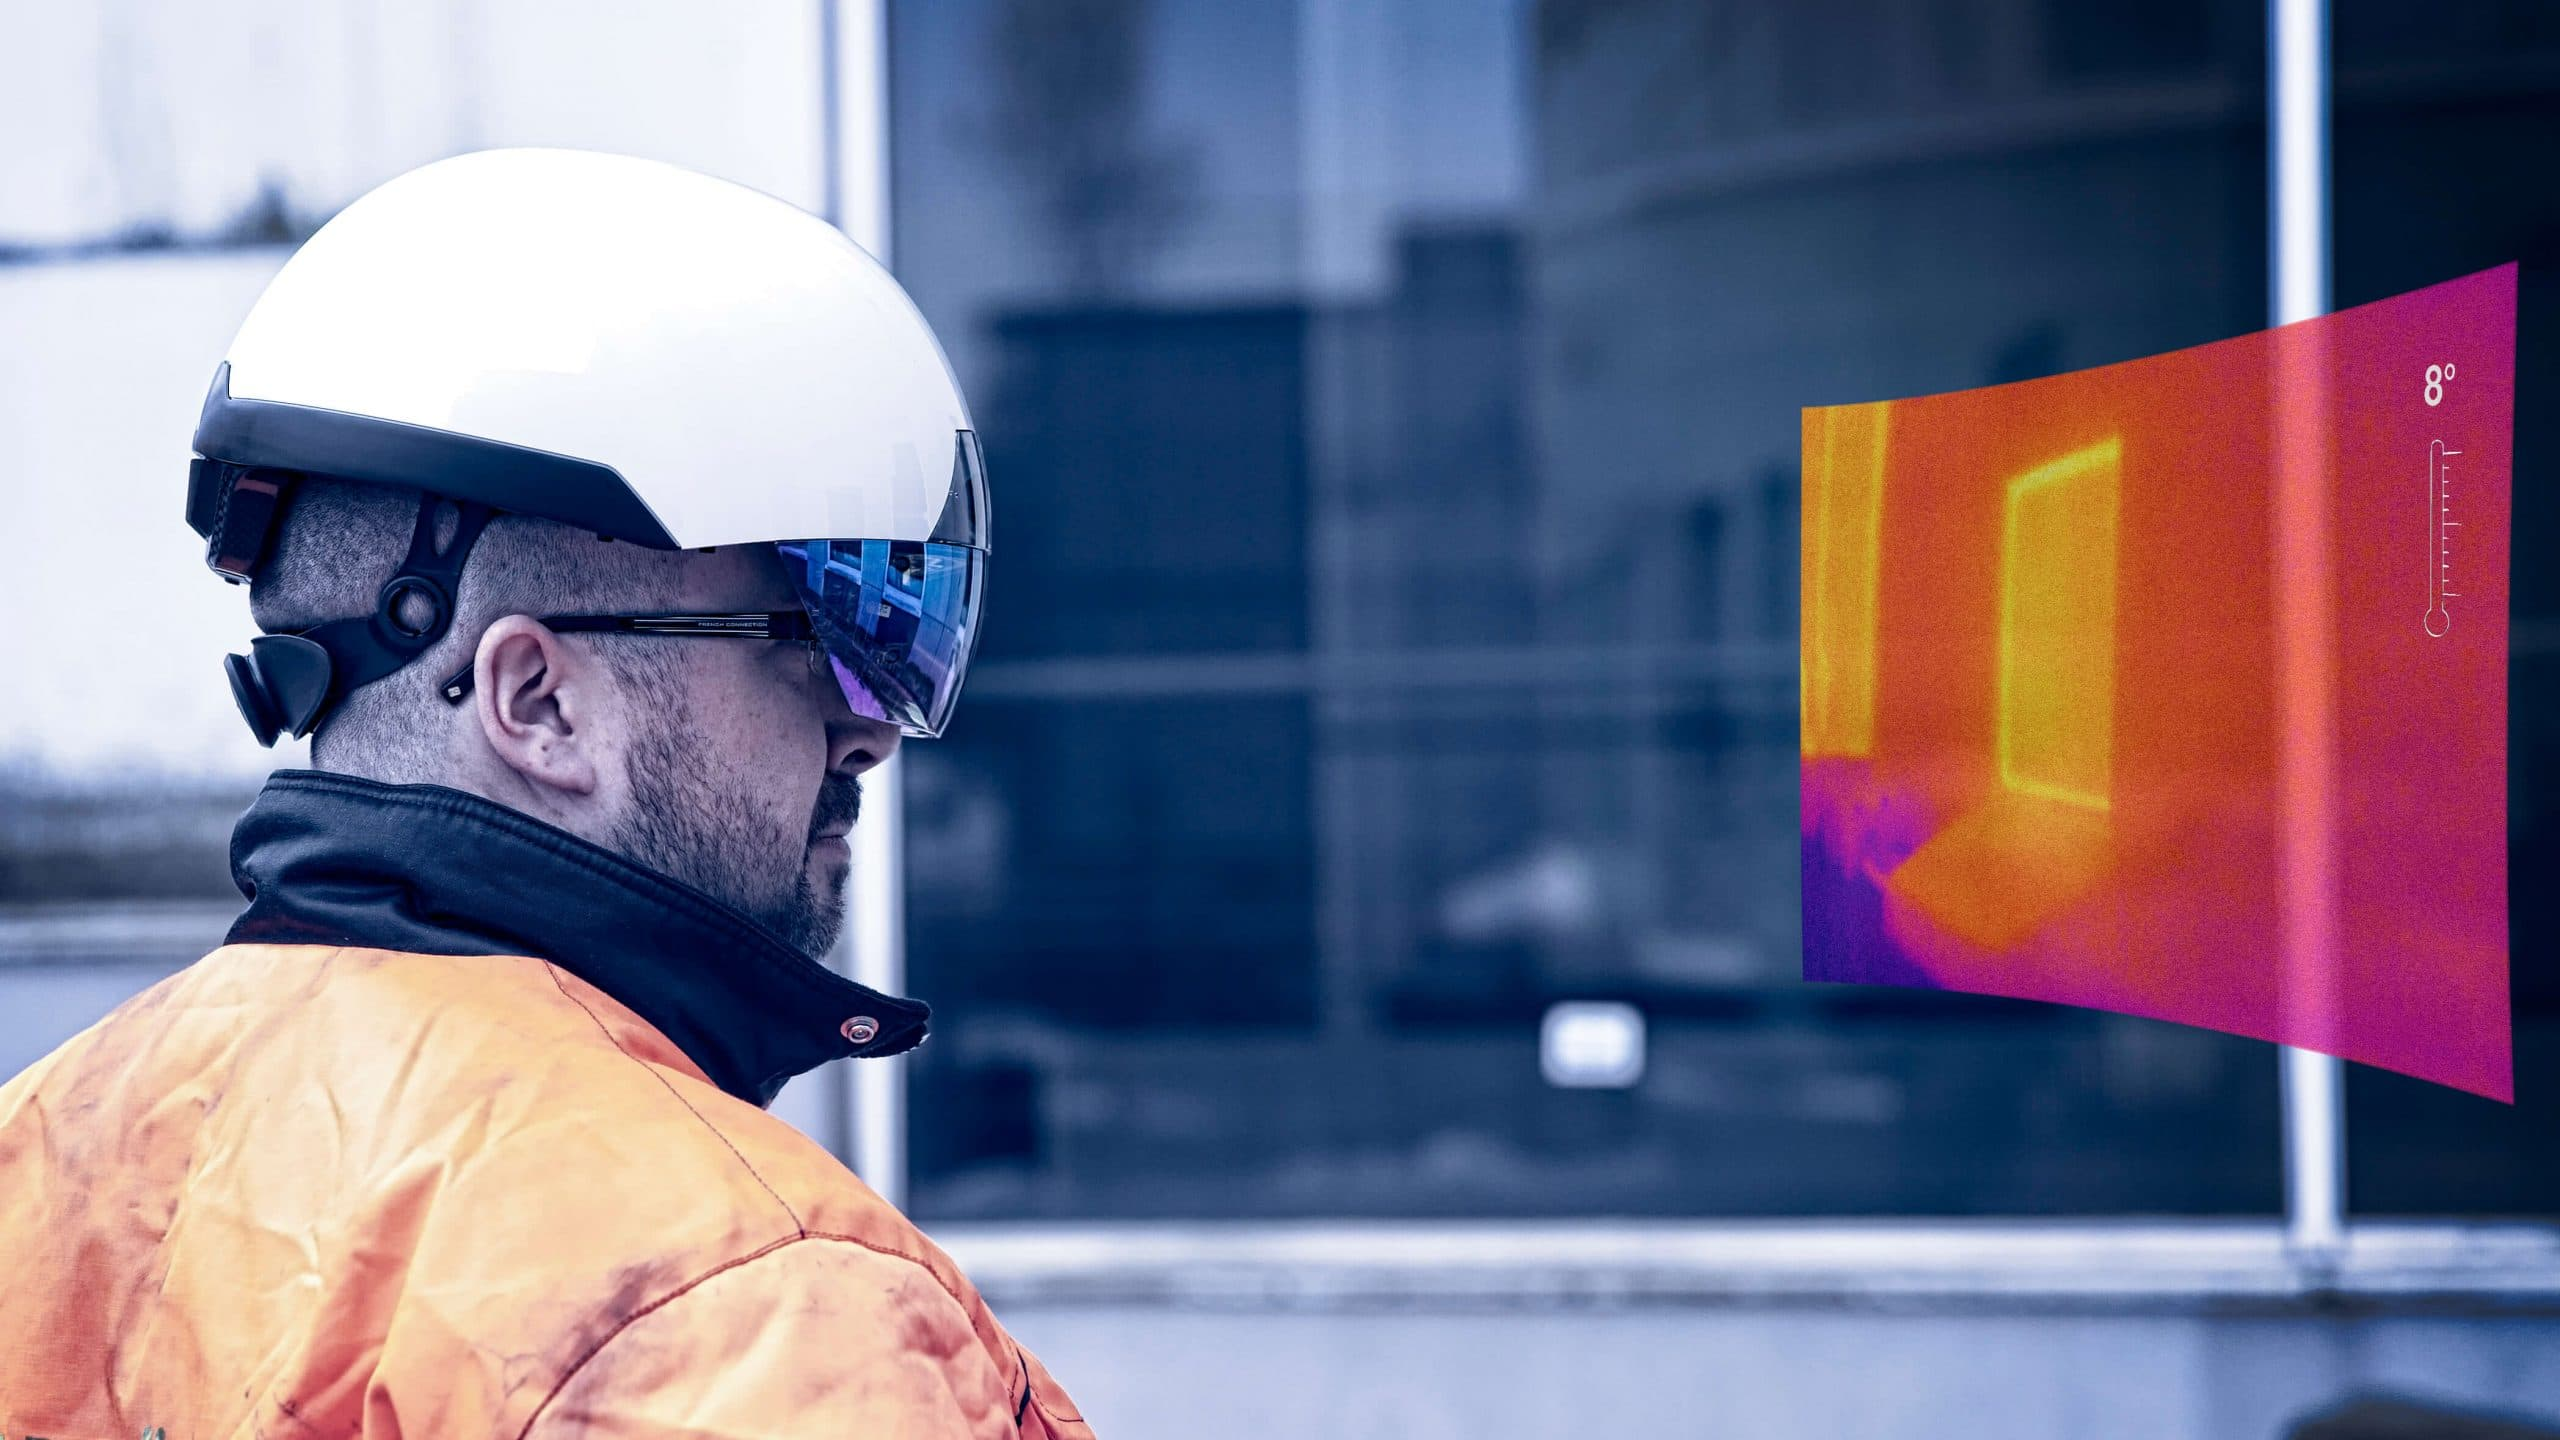
\includegraphics[scale=0.12]{Images/Estado del arte/daqrihelmet.jpg}
    \caption{Vista del DAQRI Smart Helmet}
    \label{fig:vistaDAQRIHelmet}
\end{figure}

Este modelo de DAQRI utiliza la tecnología de seguimiento SLAM (del inglés \textit{simultaneous localization and mapping}), además, tiene una cámara termográfica, barómetro, termómetro y un sensor de 9 ejes programados con algoritmos \textit{fusion hub}.\\

Por otro lado, usa unas baterías intercambiables de 5700 miliamperios por hora y no tiene tecnología de control por gestos. El precio actual del casco es de 15,000 dólares.



\footnotetext[1]{\label{daqriImagefooter}{Imagenes obtenida de: \url{https://www.stereoscape.com/blog/2017/04/25/daqri-smart-helmet-so-much-more-than-a-helmet/}.}}


